\documentclass[8pt]{beamer}

 \usepackage[utf8]{inputenc}                                                     
  \usetheme{Bergen}                                                               
%  \usecolortheme{crane}                                                       
  %\useinnertheme{circles}                                                         
  \usepackage[english]{babel}                                                     
  \usepackage{csquotes}                                                           
  \usepackage[T1]{fontenc}                                                        
  \usepackage{booktabs}                                                           
  \usepackage{amsmath}   
  \usepackage{tikz}
  \usepackage{amssymb}
  \usepackage{amsfonts}
  \usepackage{mathrsfs}   
  \usepackage{graphicx}
  \usepackage{varioref}
  \usepackage{probsoln}
  \usepackage[style=authoryear,backref=true]{biblatex}
 \usepackage[]{hyperref} 
  \graphicspath{{Graphics/}}
  \usepackage{multirow,array}
  \addbibresource{../Everything.bib}
  \usepackage{colortbl}
  \definecolor{aa}{RGB}{247, 232, 35}
  \definecolor{cc}{RGB}{29, 23, 80}    
  %\setbeamercolor{palette tertiary}{fg=aa,bg=cc}
  %\setbeamercolor{structure}{fg=cc}
  %\setbeamercolor{alerted text}{fg=red}
  
  %Information to be included in the title page:
  \title[Discrete]{AL FM Discrete}
  
  \subtitle{Critical Path Analysis: Activity Networks}
  
  \author[]{T. Bretschneider}
  
  \date[\today]{\today}

\usepackage{comment}
\usepackage{varwidth}

\newcommand{\mat}[4]{\left(\begin{array}{cc} #1 & #2 \\ #3 & #4 \\ \end{array}\right)}

\usetikzlibrary{positioning}

\def\height{0.8cm}
\def\width{1.2cm}

		\newcommand{\keynode}[6]{\node[minimum height=\height,minimum width=\width,draw,rectangle,color=aa,fill=cc] (#3) at (#1,#2) {};
	\node[rectangle,minimum height=\height/2,minimum width=\width,above,color=aa,fill=cc] at (#3) {#3};
	\node[draw,rectangle,minimum height=\height/2,minimum width=\width/3,below,color=aa,fill=cc,inner sep =0cm] at (#3) {\footnotesize#4};
	\node[draw,rectangle,minimum height=\height/2,minimum width=\width/3,below,xshift=\height/2,color=aa,fill=cc,inner sep=0cm] at (#3) {\footnotesize#5};
	\node[draw,rectangle,minimum height=\height/2,minimum width=\width/3,below,xshift=-\height/2,color=aa,fill=cc,inner sep=0cm] at (#3) {\footnotesize#6}; }



\begin{document}

\frame{\titlepage}

\begin{frame}
\frametitle{Outline}
\tableofcontents

\end{frame}

\begin{frame}{Eating Breakfast}

\begin{center}
	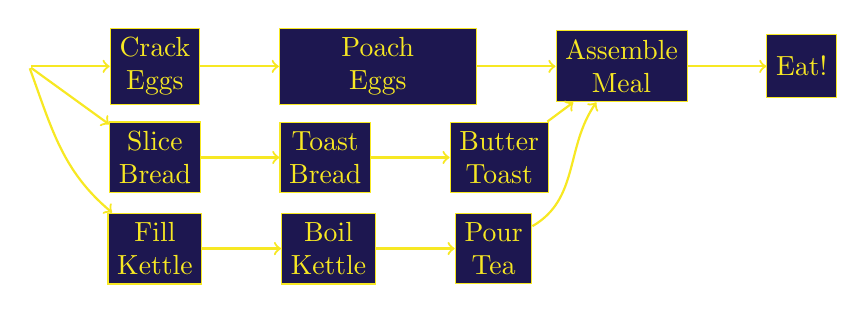
\begin{tikzpicture}
\node[inner sep=0] (A)  {};
\node[right  =of A, rectangle, draw, minimum height=0.8cm,align=center, color=aa,fill= cc] (B) {Crack\\ Eggs};
\node[below  = 0.7cm, rectangle, draw, minimum height=0.8cm,align=center, color=aa,fill= cc] (C) at (B) {Slice \\ Bread};
\node[below  =0.7cm, rectangle, draw, minimum height=0.8cm,align=center, color=aa,fill= cc] (D) at (C) {Fill \\ Kettle};
\node[right  =of B, rectangle, draw, minimum height=0.8cm,align=center, color=aa,fill= cc,minimum width=2.5cm] (E) {Poach \\Eggs};
\node[right  =of C, rectangle, draw, minimum height=0.8cm,align=center, color=aa,fill= cc] (F) {Toast \\ Bread};
\node[right  =of D, rectangle, draw, minimum height=0.8cm,align=center, color=aa,fill= cc] (G) {Boil \\ Kettle};
\node[right  =of E, rectangle, draw, minimum height=0.8cm,align=center, color=aa,fill= cc] (H) {Assemble \\ Meal};
\node[right  =of F, rectangle, draw, minimum height=0.8cm,align=center, color=aa,fill= cc] (I) {Butter \\ Toast};
\node[right  =of G, rectangle, draw, minimum height=0.8cm,align=center, color=aa,fill= cc] (J) {Pour \\ Tea};
\node[right  =of H, rectangle, draw, minimum height=0.8cm,align=center, color=aa,fill= cc] (K) {Eat!};

\draw[color=aa,->,thick] (A) -- (B); 
\draw[color=aa,->,thick] (A) -- (C); 
\draw[color=aa,->,thick] (A) to [in=140,out=290] (D); 
\draw[color=aa,->,thick] (B) -- (E); 
\draw[color=aa,->,thick] (C) -- (F); 
\draw[color=aa,->,thick] (D) -- (G); 
\draw[color=aa,->,thick] (E) -- (H); 
\draw[color=aa,->,thick] (F) -- (I); 
\draw[color=aa,->,thick] (G) -- (J); 
\draw[color=aa,->,thick] (H) -- (K); 
\draw[color=aa,->,thick] (I) -- (H); 
\draw[color=aa,->,thick] (J) to [in=235,out=30] (H); 

\end{tikzpicture}
\end{center}


	You want to make and eat your breakfast in the shortest time possible.
	
	\begin{problem}
		Why should you crack the eggs immediately.
	\end{problem}
	
	\begin{solution}<2->
		Because without cracking the eggs you can’t start poaching them and this will put back the time of assembling and eating the meal.
	\end{solution}

	\begin{problem}
		Why is there some flexibility in when you start slicing the bread.
		
	\end{problem}

	\begin{solution}<3->
		Because as long as the toast is buttered in time to assemble the meal then it doesn't.
		
	\end{solution}
\end{frame}

\begin{frame}[allowframebreaks]{Precedence Table and Activity Networks}

\begin{definition}
	A \textbf{precedence table} shows the duration of activities and their dependence on each other. 
\end{definition}

\begin{center}
	\colorbox{cc!30}{
		\setlength\arrayrulewidth{0.5mm}
		\arrayrulecolor{white}
		\begin{tabular}{ccc}
			Activity & Immediately preceding activities & Duration / hours \\
			\hline
			A &  $-$ & 4 \\
			B &  $-$ & 5 \\
			C &  A,B & 6 \\
			D &  B & 2 \\
			E &  C & 4 \\
			F &  C,D & 3 \\
		\end{tabular}
	}
	
\end{center}

\begin{definition}
	We can translate a precedence table into an \textbf{activity network} where the directed arcs represent a dependence on a preceding activity. 
	
\end{definition}


\begin{center}
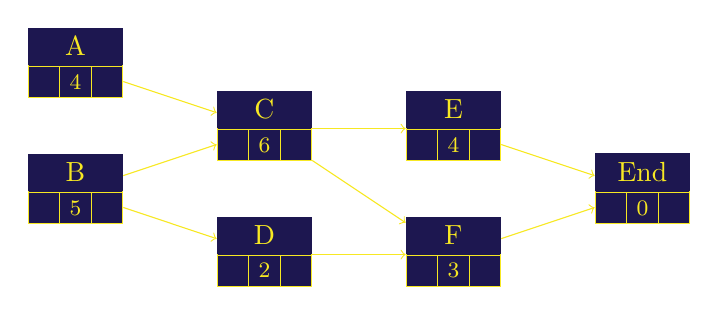
\begin{tikzpicture}
\keynode{0}{0}{A}{4}{}{}
\keynode{0}{-2*\height}{B}{5}{ }{}
\keynode{2*\width}{-\height}{C}{6}{}{}
\keynode{2*\width}{-3*\height}{D}{2}{}{}
\keynode{4*\width}{-\height}{E}{4}{}{}
\keynode{4*\width}{-3*\height}{F}{3}{}{}
\keynode{6*\width}{-2*\height}{End}{0}{}{}

\draw[->,color=aa] (A) --  (C);
\draw[->,color=aa] (B) --  (C);
\draw[->,color=aa] (B) --  (D);
\draw[->,color=aa] (C) --  (E);
\draw[->,color=aa] (C) --  (F);
\draw[->,color=aa] (D) --  (F);
\draw[->,color=aa] (E) --  (End);
\draw[->,color=aa] (F) --  (End);
\end{tikzpicture}
\end{center}

\alert{Note that the middle box is for the duration and we shall see that the left and right boxes are for the earliest start time and latest finish time respectively.}
	
\end{frame}

\begin{frame}{Determining Earliest Start Times}
	\begin{definition}
		Make a 'forward pass' through the network moving onto an activity when all of its preceding activities have been completed.

		The \textbf{earliest start time} is the  maximum of the earliest start times $+$ duration of all the preceding actives.
	\end{definition}


\begin{center}
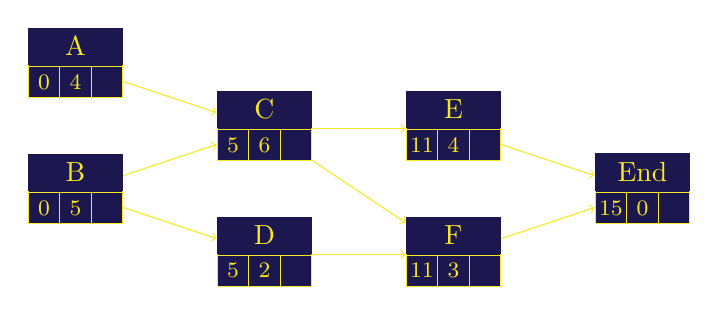
\begin{tikzpicture}
\keynode{0}{0}{A}{4}{}{0}
\keynode{0}{-2*\height}{B}{5}{ }{0}
\keynode{2*\width}{-\height}{C}{6}{}{5}
\keynode{2*\width}{-3*\height}{D}{2}{}{5}
\keynode{4*\width}{-\height}{E}{4}{}{11}
\keynode{4*\width}{-3*\height}{F}{3}{}{11}
\keynode{6*\width}{-2*\height}{End}{0}{}{15}

\draw[->,color=aa] (A) --  (C);
\draw[->,color=aa] (B) --  (C);
\draw[->,color=aa] (B) --  (D);
\draw[->,color=aa] (C) --  (E);
\draw[->,color=aa] (C) --  (F);
\draw[->,color=aa] (D) --  (F);
\draw[->,color=aa] (E) --  (End);
\draw[->,color=aa] (F) --  (End);
\end{tikzpicture}
\end{center}

Activities that don't depend on any others can all start at the beginning and hence get a 0 in the 'Earliest Start Time' box.

The minimum completion time for this activity is therefore 15 hours.

\end{frame}

\begin{frame}{Determining the Latest Finish Times}
	\begin{block}{Method}
		We now make a 'backward' pass through the network to find the latest finish times if we are to complete the task in the minimum completion time.

		Starting at the end, the latest finish time is the minimum of the latest finish time of any dependent activities subtract their duration. 
	\end{block}




\begin{center}
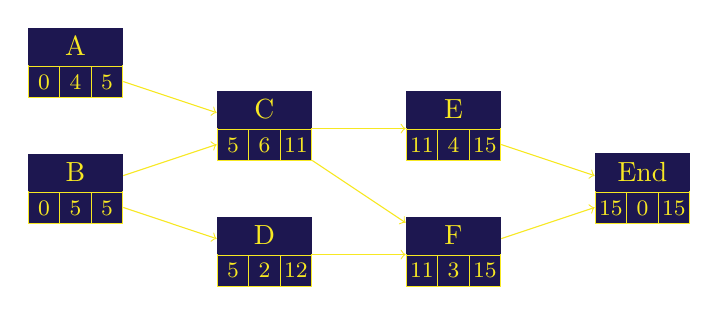
\begin{tikzpicture}
\keynode{0}{0}{A}{4}{5}{0}
\keynode{0}{-2*\height}{B}{5}{5}{0}
\keynode{2*\width}{-\height}{C}{6}{11}{5}
\keynode{2*\width}{-3*\height}{D}{2}{12}{5}
\keynode{4*\width}{-\height}{E}{4}{15}{11}
\keynode{4*\width}{-3*\height}{F}{3}{15}{11}
\keynode{6*\width}{-2*\height}{End}{0}{15}{15}

\draw[->,color=aa] (A) --  (C);
\draw[->,color=aa] (B) --  (C);
\draw[->,color=aa] (B) --  (D);
\draw[->,color=aa] (C) --  (E);
\draw[->,color=aa] (C) --  (F);
\draw[->,color=aa] (D) --  (F);
\draw[->,color=aa] (E) --  (End);
\draw[->,color=aa] (F) --  (End);
\end{tikzpicture}
\end{center}


\end{frame}

\begin{frame}[allowframebreaks]{Float}
\begin{definition}
	The \textbf{float} of an activity is the 'slack time'
	\[
		\text{Float} = (\text{Latest Finish Time} - \text{Earlies Start Time}) - \text{Duration}
	.\] 
	
\end{definition}	

\begin{definition}
	If an activity has no float it is called \textbf{critical}. In other words, if the activity is to finish in the minimum completion time, there is no flexibility about when this activity starts.
	
\end{definition}

\begin{columns}
	\begin{column}{0.6\textwidth}

\begin{center}
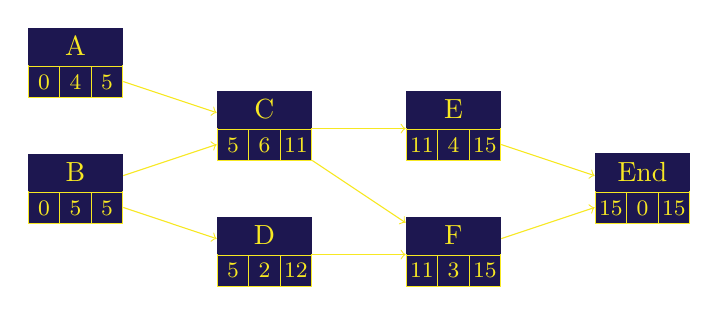
\begin{tikzpicture}
\keynode{0}{0}{A}{4}{5}{0}
\keynode{0}{-2*\height}{B}{5}{5}{0}
\keynode{2*\width}{-\height}{C}{6}{11}{5}
\keynode{2*\width}{-3*\height}{D}{2}{12}{5}
\keynode{4*\width}{-\height}{E}{4}{15}{11}
\keynode{4*\width}{-3*\height}{F}{3}{15}{11}
\keynode{6*\width}{-2*\height}{End}{0}{15}{15}

\draw[->,color=aa] (A) --  (C);
\draw[->,color=aa] (B) --  (C);
\draw[->,color=aa] (B) --  (D);
\draw[->,color=aa] (C) --  (E);
\draw[->,color=aa] (C) --  (F);
\draw[->,color=aa] (D) --  (F);
\draw[->,color=aa] (E) --  (End);
\draw[->,color=aa] (F) --  (End);
\end{tikzpicture}
\end{center}



		
	\end{column}
	\begin{column}{0.4\textwidth}
		

\begin{center}
	\colorbox{cc!30}{
		\setlength\arrayrulewidth{0.5mm}
		\arrayrulecolor{white}
		\begin{tabular}{ccc}
			Activity & Float & Critical \\
			\hline
			A &  1 & No \\
			B &  0 & Yes \\
			C &  0 & Yes \\
			D &  5 & No \\
			E &  0 & Yes \\
			F &  1 & No \\
		\end{tabular}
	}
	
\end{center}
	\end{column}
\end{columns}

\begin{definition}
	The critical activities for the \textbf{critical path} through the network. The length of the \textbf{critical path} is the minimum completion time of the project. Such a critical path will always exist, although there may be more than one but all critical paths will have the same length. 
	
\end{definition}

\end{frame}

\begin{frame}{Project Management}
	\begin{itemize}
		\item The non-critical activities don’t have to be undertaken in their minimum duration. This
means that their duration can be increased without affecting the overall completion
time of the project which will often decrease costs.
\item More resource (e.g. more workers) can be invested in the critical activities, reducing
their duration and speeding up the overall completion time.
	\end{itemize}
\end{frame}

\begin{frame}{Reducing Cost}
	\begin{problem}
		What is the minimum extra cost from the original planned duration of this project so that it can be completed as quickly as possible?

		

\begin{center}
	\colorbox{cc!30}{
		\setlength\arrayrulewidth{0.5mm}
		\arrayrulecolor{white}
		\begin{tabular}{c>{\centering\arraybackslash}m{2cm}>{\centering\arraybackslash}m{2cm}>{\centering\arraybackslash}m{2.2cm}>{\centering\arraybackslash}m{2cm}}
	Activity & Immediately preceding activities & Original Duration (in hours) & Cost of reducing duration by 1 hour & Minimum duration possible \\
	\hline
	A &  & 4 & 100 & 2 \\
	B &  & 5 & 200 & 4 \\
	C & A,B & 6 & 100 & 3 \\
	D & B & 2 & 300 & 1 \\
	E & C & 4 & 200 & 1 \\
	F & C,D & 5 & 200 & 2 \\
\end{tabular}
	}
	
\end{center}
	\end{problem}
	\begin{solution}
		Activity network with the minimum duration:


\begin{center}
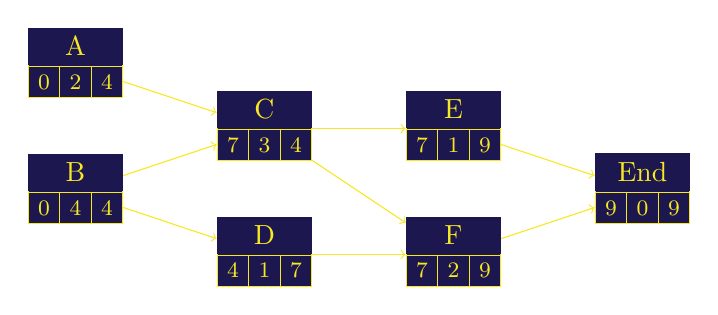
\begin{tikzpicture}
\keynode{0}{0}{A}{2}{4}{0}
\keynode{0}{-2*\height}{B}{4}{4}{0}
\keynode{2*\width}{-\height}{C}{3}{4}{7}
\keynode{2*\width}{-3*\height}{D}{1}{7}{4}
\keynode{4*\width}{-\height}{E}{1}{9}{7}
\keynode{4*\width}{-3*\height}{F}{2}{9}{7}
\keynode{6*\width}{-2*\height}{End}{0}{9}{9}

\draw[->,color=aa] (A) --  (C);
\draw[->,color=aa] (B) --  (C);
\draw[->,color=aa] (B) --  (D);
\draw[->,color=aa] (C) --  (E);
\draw[->,color=aa] (C) --  (F);
\draw[->,color=aa] (D) --  (F);
\draw[->,color=aa] (E) --  (End);
\draw[->,color=aa] (F) --  (End);
\end{tikzpicture}
\end{center}

The floats are, A2,B0,C0,D2,E1,F0

Now calculate the extra costs to complete the activities in these durations for the minimum completion time compared to the original planned duration.



\begin{center}
	\colorbox{cc!30}{
		\setlength\arrayrulewidth{0.5mm}
		\arrayrulecolor{white}
		\begin{tabular}{c>{\centering\arraybackslash}m{1.5cm}>{\centering\arraybackslash}m{1.3cm}}
	Activity & New Duration & Extra Cost \\
	\hline
	A & 4 & 0 \\
	B & 4 & 200 \\
	C & 3 & 300 \\
	D & 2 & 0 \\
	E & 2 & 400 \\
	F & 2 & 200 \\
\end{tabular}
	}
	
\end{center}
So the total extra cost is 1100.
	\end{solution}
\end{frame}

\begin{frame}[allowframebreaks]{Past Paper Question}
	\begin{problem}
		Deva Construction Ltd undertakes a small building project. 

		\begin{center}
			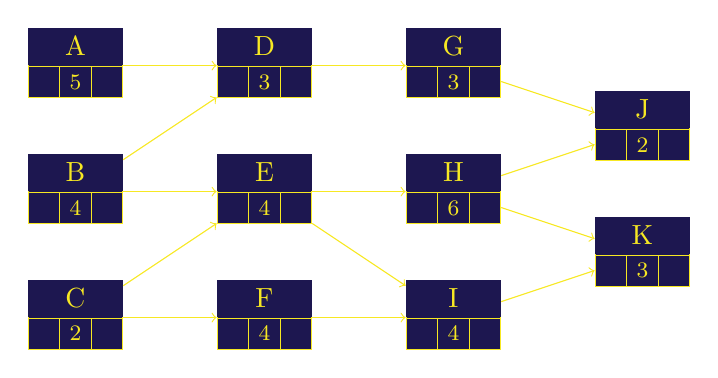
\begin{tikzpicture}
				\keynode{0}{0}{A}{5}{}{}
				\keynode{0}{-2*\height}{B}{4}{}{}
				\keynode{0}{-4*\height}{C}{2}{}{}
				\keynode{2*\width}{0}{D}{3}{}{}
				\keynode{2*\width}{-2*\height}{E}{4}{}{}
				\keynode{2*\width}{-4*\height}{F}{4}{}{}
				\keynode{4*\width}{0}{G}{3}{}{}
				\keynode{4*\width}{-2*\height}{H}{6}{}{}
				\keynode{4*\width}{-4*\height}{I}{4}{}{}
				\keynode{6*\width}{-1*\height}{J}{2}{}{}
				\keynode{6*\width}{-3*\height}{K}{3}{}{}
	
				\draw[->,color=aa] (A) -- (D);		
				\draw[->,color=aa] (B) -- (D);		
				\draw[->,color=aa] (B) -- (E);		
				\draw[->,color=aa] (C) -- (E);		
				\draw[->,color=aa] (C) -- (F);		
				\draw[->,color=aa] (D) -- (G);		
				\draw[->,color=aa] (E) -- (H);		
				\draw[->,color=aa] (E) -- (I);		
				\draw[->,color=aa] (F) -- (I);		
				\draw[->,color=aa] (G) -- (J);		
				\draw[->,color=aa] (H) -- (J);		
				\draw[->,color=aa] (H) -- (K);		
				\draw[->,color=aa] (I) -- (K);		
			\end{tikzpicture}
			
		\end{center}

		\begin{itemize}
			\item Complete the activity network for the building project.
			\item Deva Construction Ltd is able to reduce the duration of a single activity to 1 hour by using specialist equipment.

				State, with a reason, which activity should have its duration reduced to 1 hour in order to minimise the completion time for the building project.
			\item State one limitation in the building project used by Deva Construction ltd.

				Explain how this limitation affect the project.
		\end{itemize}

	\end{problem}

\begin{solution}<2->
	

		\begin{center}
			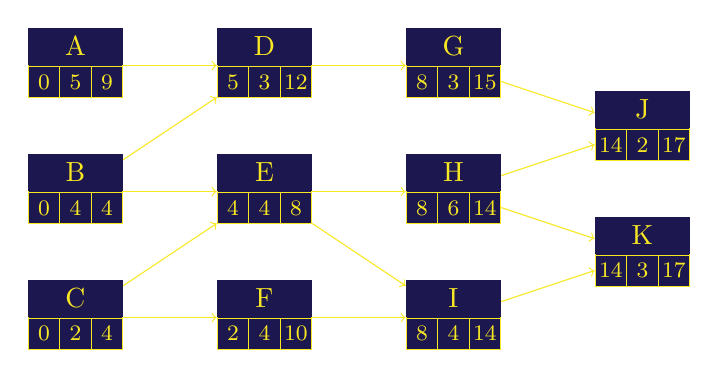
\begin{tikzpicture}
				\keynode{0}{0}{A}{5}{9}{0}
				\keynode{0}{-2*\height}{B}{4}{4}{0}
				\keynode{0}{-4*\height}{C}{2}{4}{0}
				\keynode{2*\width}{0}{D}{3}{12}{5}
				\keynode{2*\width}{-2*\height}{E}{4}{8}{4}
				\keynode{2*\width}{-4*\height}{F}{4}{10}{2}
				\keynode{4*\width}{0}{G}{3}{15}{8}
				\keynode{4*\width}{-2*\height}{H}{6}{14}{8}
				\keynode{4*\width}{-4*\height}{I}{4}{14}{8}
				\keynode{6*\width}{-1*\height}{J}{2}{17}{14}
				\keynode{6*\width}{-3*\height}{K}{3}{17}{14}
	
				\draw[->,color=aa] (A) -- (D);		
				\draw[->,color=aa] (B) -- (D);		
				\draw[->,color=aa] (B) -- (E);		
				\draw[->,color=aa] (C) -- (E);		
				\draw[->,color=aa] (C) -- (F);		
				\draw[->,color=aa] (D) -- (G);		
				\draw[->,color=aa] (E) -- (H);		
				\draw[->,color=aa] (E) -- (I);		
				\draw[->,color=aa] (F) -- (I);		
				\draw[->,color=aa] (G) -- (J);		
				\draw[->,color=aa] (H) -- (J);		
				\draw[->,color=aa] (H) -- (K);		
				\draw[->,color=aa] (I) -- (K);		
			\end{tikzpicture}
			
		\end{center}

\end{solution}

\begin{solution}<3->
	Reducing the duration of activity E to 1 reduces the project completion time to 14 hours, whereas all other activities reduce the project completion time to 15 hours or more.
\end{solution}

\begin{solution}<4->
	Time between one activity ending and the next starting is not taken into account, as workers may need to travel to a different location.

	The travelling time will cause subsequent activities to be delayed, increasing the project completion time.
\end{solution}

\end{frame}
\end{document}
